

\documentclass[color=usenames,dvipsnames]{beamer}

\usepackage[adobefonts,noindent]{ctex} %中文支持
\setCJKmainfont{SimSun}

\mode<presentation> {

\usetheme{Madrid}
\usecolortheme{lily}
\useoutertheme{infolines}

}


\usepackage{booktabs} 
\usepackage{tikz}


% Thin fonts
\usepackage{cmbright}
\usepackage[T1]{fontenc}

\definecolor{dark_grey}{gray}{0.5}
\setbeamercolor{normal text}{fg=dark_grey,bg=white}
\setbeamertemplate{navigation symbols}{}

\setbeamercolor*{palette primary}{fg=gray!100,bg=gray!10}
\setbeamercolor*{palette quaternary}{fg=gray!100,bg=gray!10}
\setbeamercolor*{palette secondary}{fg=gray!100,bg=gray!20}
\setbeamercolor*{palette tertiary}{fg=gray!100,bg=gray!10}
\setbeamercolor*{navigation symbols}{fg=white,bg=white}
\usefonttheme{default}


\setbeamertemplate{blocks}[rounded][shadow=false]
\setbeamercolor{block title}{bg=gray!10}
\setbeamercolor{block body}{fg=gray,bg=gray!10}
%\setbeamercolor{frametitle}{fg=}

\setbeamertemplate{frametitle}[default][center]

\setbeamertemplate{itemize items}[default]
\setbeamertemplate{enumerate items}[default]

\newcommand{\F}{\mathbb{F}}


\title[KBText Embed]{Representing Text for Joint Embedding of Text and Knowledge Bases}
\subtitle{Kristina Toutanova@MS\\ Danqi Chen@Stanford\\ EMNLP2015}
\author{韩喆}
\institute{ICSTWIP}
\date{20160107}
\begin{document}


\begin{frame}
  \titlepage
\end{frame}

% Uncomment these lines for an automatically generated outline.
%\begin{frame}{Outline}
%  \tableofcontents
%\end{frame}

\begin{frame}{outline}
 \begin{itemize}
  \item 作者简介
  \item 问题定义:Knowledge Base + 文本抽取新关系
  \item 相关工作:KBC、文本、混合模型
  \item 实验
    \begin{itemize}
     \item 模型介绍
     \item 实验结果
    \end{itemize}
 \end{itemize}

\end{frame}

\begin{frame}{作者简介}\footnotesize
  \begin{columns}
   \column{0.3\hsize}
   \begin{center}
     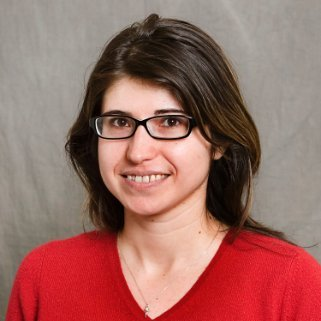
\includegraphics[width=0.65\hsize]{pic/kristina2.jpg}
   \end{center}
     \begin{block}{}
      \begin{itemize}
       \item 保加利亚/美国人?
       \item Sofia-Uni -> stanford.NLP -> MS
       \item 句法语法分析,MT,摘要,...都做
      \end{itemize}
     \end{block}

   \column{0.3\hsize}
   \begin{center}
     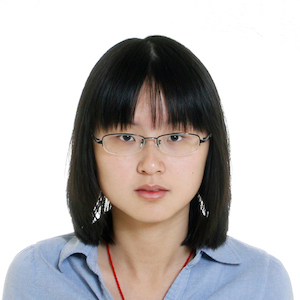
\includegraphics[width=0.65\hsize]{pic/danqi2.jpg}
   \end{center}
     \begin{block}{}
      \begin{itemize}
       \item THU.Yao -> stanford.NLP
       \item DL,NLP
      \end{itemize}
     \end{block}
     
   \column{0.35\hsize}
   \begin{columns}
   \column{0.3\hsize}
   \alert{\textbf{ 相关人物,非作者: }}
   \column{0.8\hsize}
   \begin{center}
     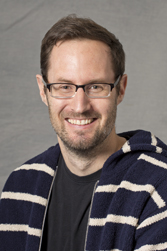
\includegraphics[width=0.35\hsize]{pic/Riedel.jpg}
   \end{center}
   \end{columns}
     \begin{block}{}
      \begin{itemize}
       \item Phd@Edinburgh -> researcher@UTokyo -> researcher@umass -> AP@UCL.Machine Reading Lab
       \item 机器阅读,NLP
       \item 主页放了一个叫Mika Riedel的日本女生的绘画/雕刻作品,貌似是他老婆?
      \end{itemize}
     \end{block}
  \end{columns}

\end{frame}


\section{Introduction}

\begin{frame}{任务简介}

\only<1-2>{
  \begin{itemize}
   \item 给定RDF知识库$KB=\{(e_s,r,e_o),...\}$
   \item 问KB中没有的关系,找出最合适的实体:$(e_s,r,?),(?,r,e_o)$
    \begin{itemize}
     \item 类似的还有$(e_s,?,e_o)$,这里面候选$r$可能有多个?
     \item 本文认为候选只有一个?
     \item 本文只对第一个效果进行实验
    \end{itemize}

   \only<2>{\alert{
      \item $e_o=\arg \max\limits_{e_j} f((e_s,r,e_j))$
      \item $f((e_s,r,e_o)) = f_2(v_{e_s},v_{r},v_{e_o})$
	\begin{itemize}
	 \item 一个好的语义向量$\mathcal{R}=\{r_1,r_2,...\},\mathcal{E}=\{e_1,e_2,...\}$
	 \item 一个好的模型$f_2$
	\end{itemize}
   }}
   
  \end{itemize}

}


\only<3->{
 \begin{itemize}
  \item 基于Riedel 13 年的文章,从KB+text中抽取语义向量(实体的向量,关系的向量),做关系预测\\ 
    \begin{footnotesize}
     Relation extraction with matrix factorization and universal schemas
    \end{footnotesize}
  \begin{itemize}
   \item 将text中的dependency path作为实体的“新关系”,增大图的密集程度(关系数量显著增加)
  \end{itemize}
 \end{itemize}
 
 \begin{columns}
  \column{0.7\hsize}
  \centering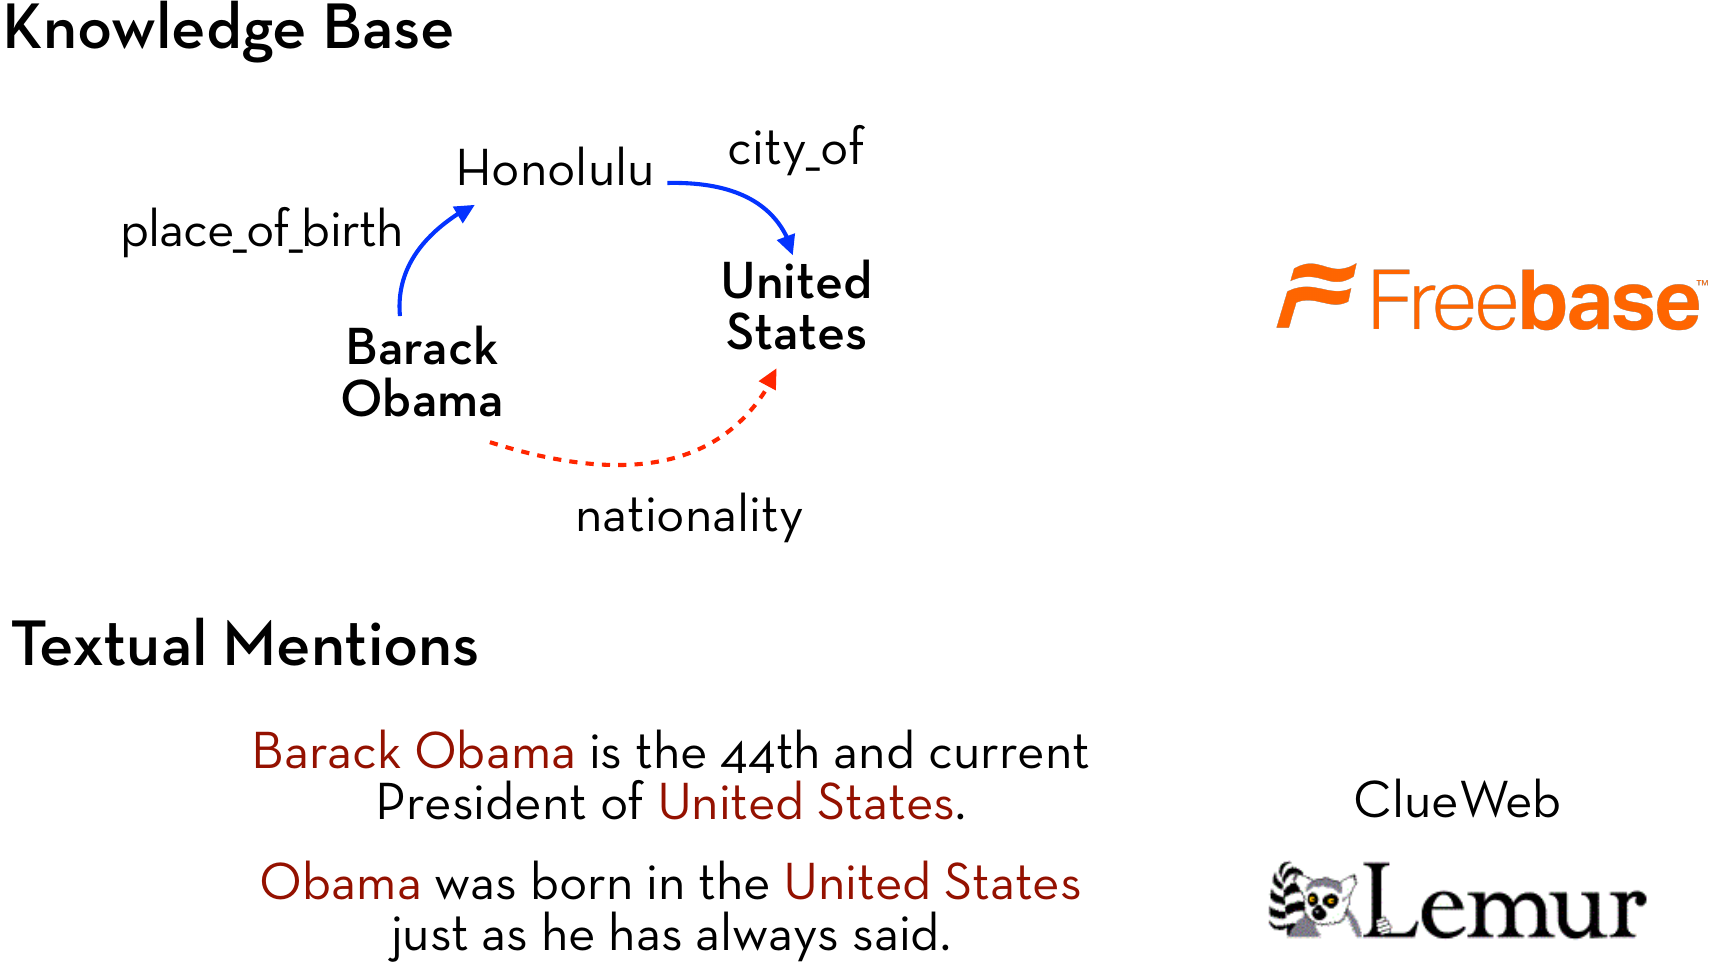
\includegraphics[width=0.95\hsize]{pic/riedel13.png}
  \column{0.3\hsize}
  \only<4>{\alert{相似的dependency path 被看成不同的“新关系”,尽管他们只有很小的差别}}
 \end{columns}
}
\end{frame}


\frame{
  \begin{columns}[c]
   \column{.15\hsize}
   \column{.7\hsize}
   \begin{block}{}
    \centering \Large 相关工作  \\ 
    \small --- Knowledge base completion \\ 
    \small --- Relation extraction using distant supervision \\ 
    \small --- Combining KB and text \\ 
   \end{block}
   \column{.15\hsize}
  \end{columns}
}


\frame{
  \frametitle{Knowledge base completion}
  \only<1>{
  \begin{itemize}
   \item 初始版的path ranking algorithm (劳逆 2011)
    \begin{itemize}
     \item 我的理解:基本想法是主语和相似实体有相同的属性/属性值,近似于双向random walk+剪枝
    \end{itemize}
  \end{itemize}
  \centering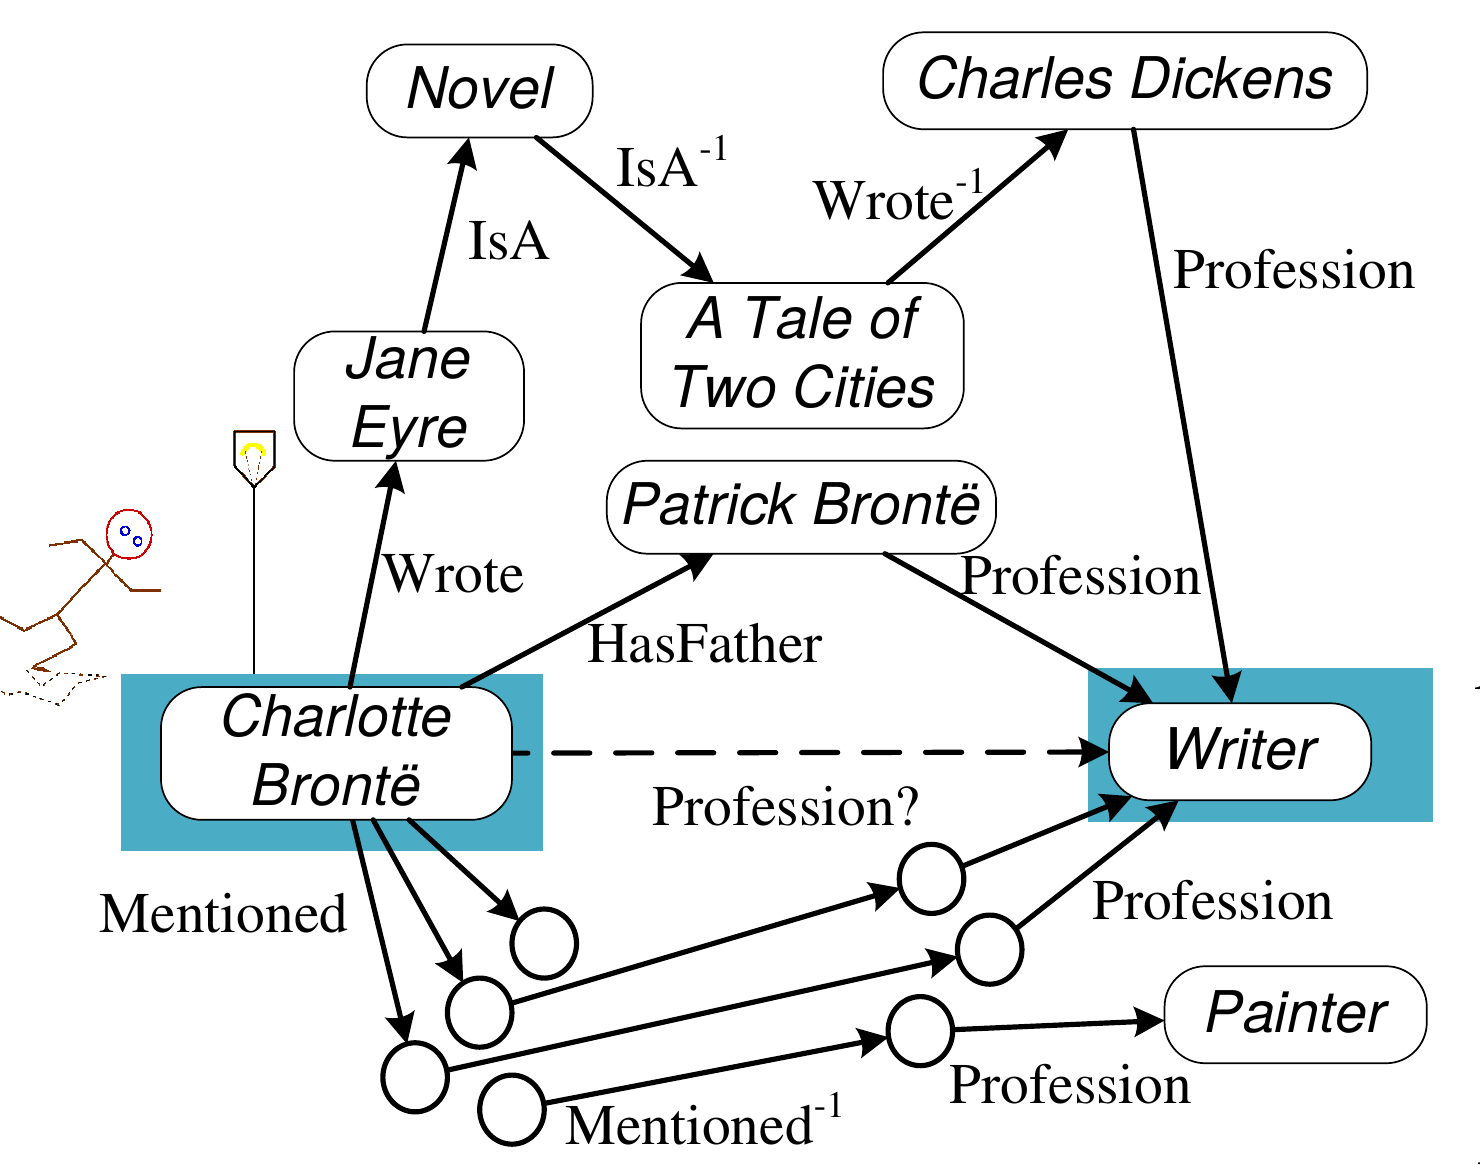
\includegraphics[width=0.55\hsize]{pic/pra.png}
  }
  
  \only<2>{
  \begin{itemize}
   \item DISTMULT (后面讲, Yang 2015)
   \item TransE (之前讲过,贴在下面)
  \end{itemize}
  \centering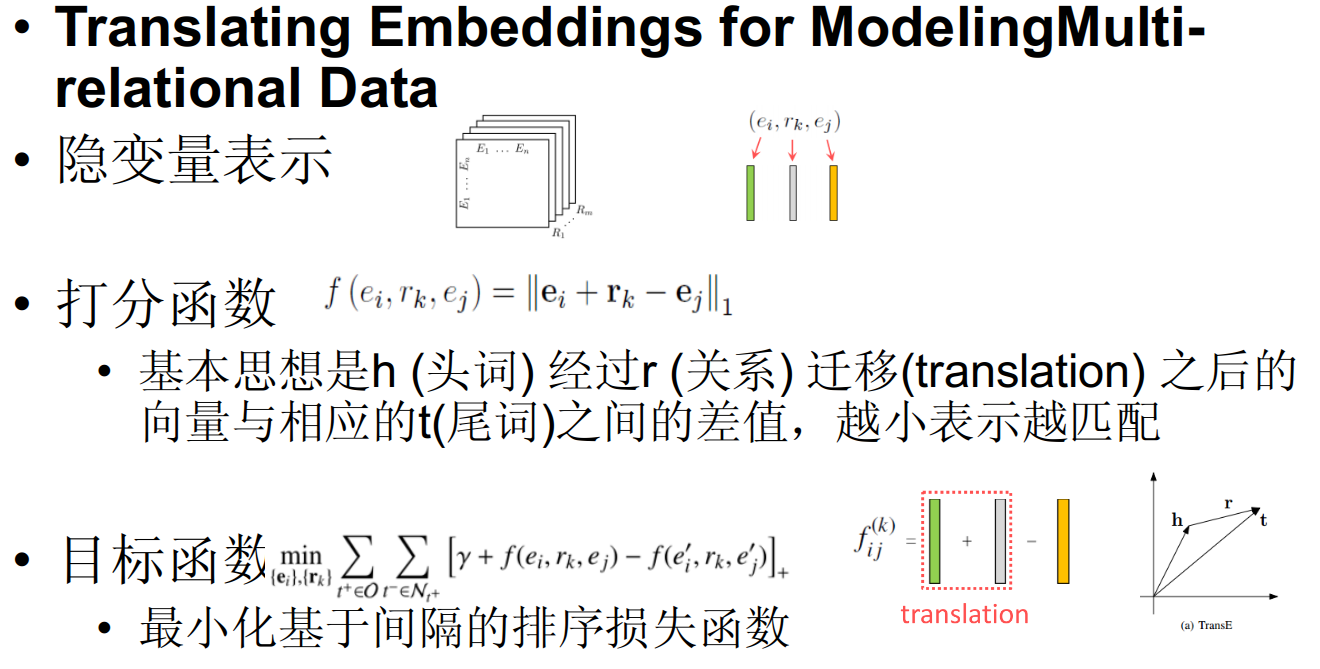
\includegraphics[width=0.8\hsize]{pic/transE.png}
  }
  
}

\frame{
  \only<1>{
  \frametitle{Relation extraction using distant supervision}
    \begin{itemize}
     \item 即单纯从文本中抽取实体的关系,不使用KB
      \begin{itemize}
       \item 使用dependency path 建立实体间的关系
       \alert{\item 没用考虑d-path里面的相同子结构}
       \item 比较老,09-11年
      \end{itemize}
    \end{itemize}
  }
  
  \only<2>{
  \frametitle{Combining knowledge base and text information}
  同时利用 KB和text来抽取新关系
    \begin{enumerate}
     \item 后来的path ranking algorithm (劳逆 2012)
      \begin{itemize}
       \item 从text中抽取text-graph(实体是点,关系是边),解决边的稀疏性问题
      \end{itemize}
     \item (Neelakantan 2015) 使用在文本中共现的实体对增加图中边
     \item 有的是训练每个实体和所有在实体中出现的单词
      \begin{itemize}
       \item 含有相似单词的实体会训练出相似的词向量?
      \end{itemize}
     \item 分别在KB和text中训练不同的词向量
     \alert{\item 没用考虑d-path里面的相同子结构}
    \end{enumerate}
  }
}



\frame{
  \begin{columns}[c]
   \column{.15\hsize}
   \column{.7\hsize}
   \begin{block}{}
    \centering \Large 模型介绍  \\ 
   \end{block}
   \column{.15\hsize}
  \end{columns}
}

\frame{
  \frametitle{目标函数}
  目标函数 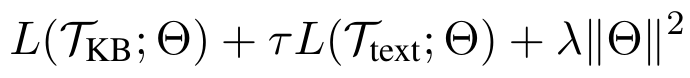
\includegraphics[width=0.45\hsize]{pic/lossFunc.png}
  \begin{itemize}
   \item 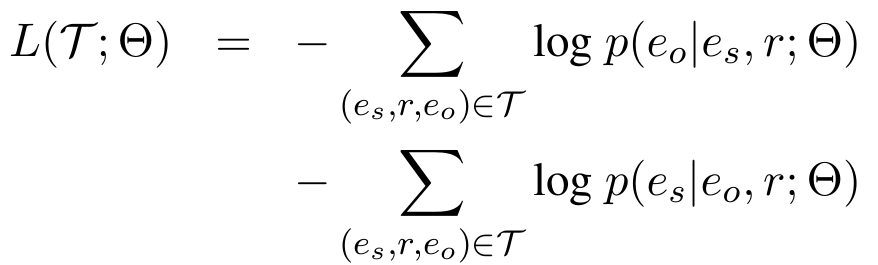
\includegraphics[width=0.55\hsize]{pic/lossFunc2.png}
   \item 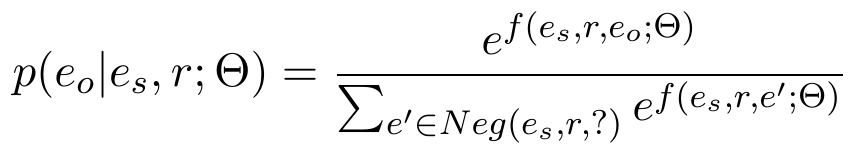
\includegraphics[width=0.45\hsize]{pic/p.png}
   \item 权重变量$\tau$手动确定,$f((e_s,r,e_o))$采用不同的模型(或他们的$f$函数的值简单相加),下面具体说明这几个$f$函数
  \end{itemize}

}
\frame{
  \frametitle{模型介绍}
  \begin{columns}
   \column{0.35\hsize}
   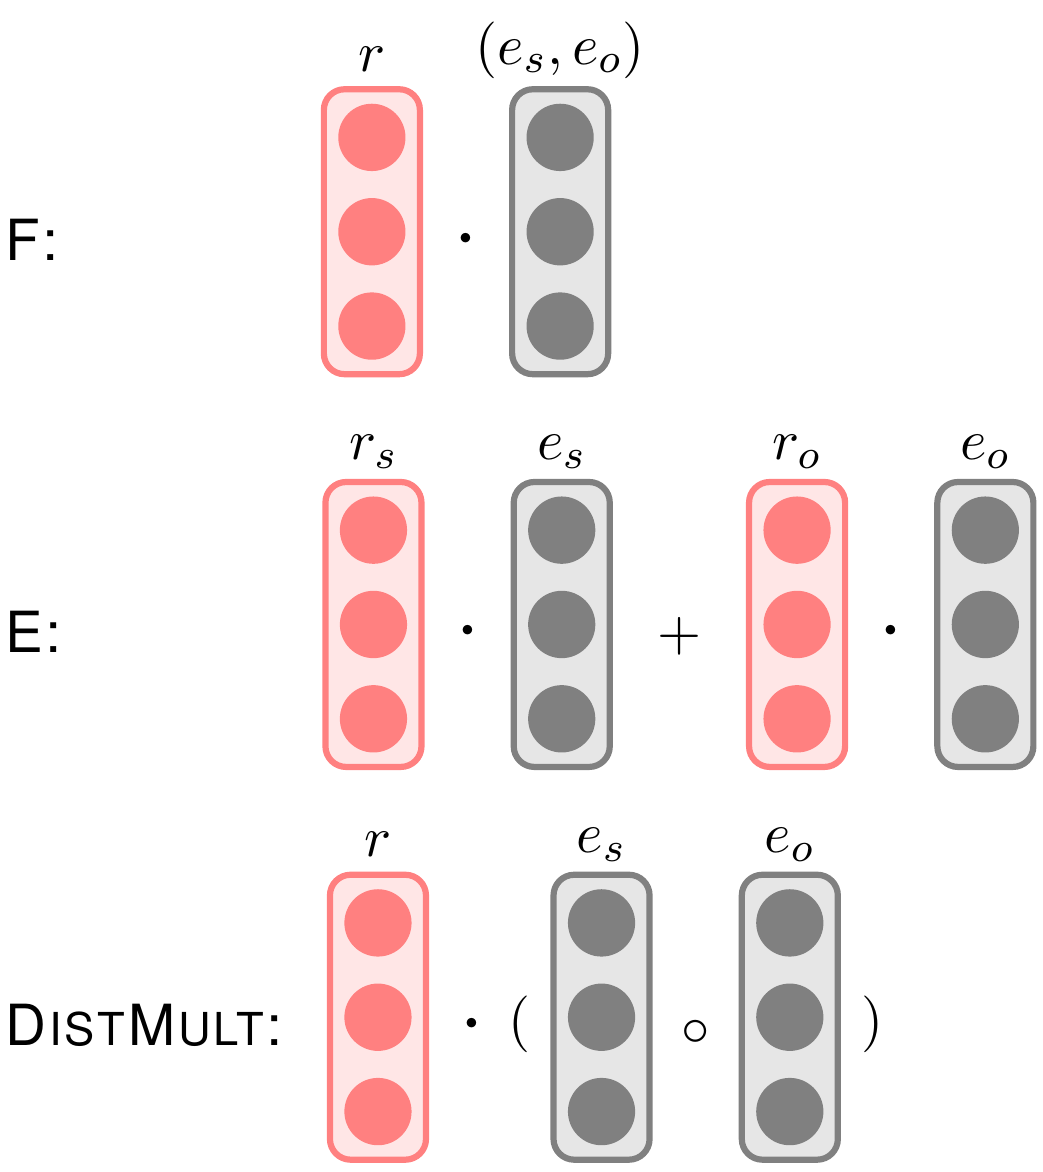
\includegraphics[width=0.95\hsize]{pic/models.png}
   
   \column{0.65\hsize}
   \only<1->{
   \begin{block}{E模型}
   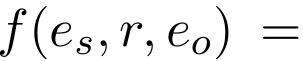
\includegraphics[width=0.35\hsize]{pic/emodel0.png}
   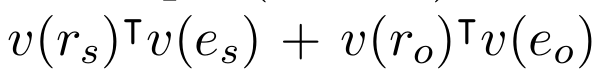
\includegraphics[width=0.5\hsize]{pic/emodel1.png}
   \end{block}
   \only<2>{
    \alert{$e_o$和$e_s$无关,只和$r$有关}
   }
   \only<3->{
   \begin{block}{DISTMULT模型}
   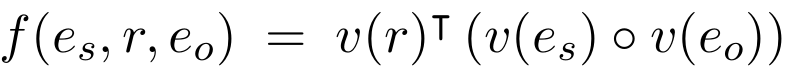
\includegraphics[width=0.95\hsize]{pic/fmodel.png}
   \end{block}
   }
   \only<4>{
    {\alert{$(e_s,r,e_o)$和$(e_s,r,e_o)$一样,学出来的$r$向量不能区分反向关系}}
    }

   \only<5->{
   复杂度,$N_e=|\mathcal{E}|,N_r=|\mathcal{R}|,K$为维度
   \begin{itemize}
    \item E:$KN_e+2KN_r$
    \item DISTMULT:$KN_e+KN_r$
    \item F:$KN_e^2+KN_r$
   \end{itemize}
   }
   }
   \only<6>{
   \alert{\textbf{E、F模型由Riedel提出,DISTMULT由Yang提出,作者直接使用}}
   }
  \end{columns}


}

\begin{frame}{模型介绍}
 CONV: Compositional Representations of Textual Relations
 \begin{itemize}
  \item 为了解决从句子中抽取关系时两个很相似的实体对所使用的d-path被当成不同的关系
    \begin{itemize}
     \item 过去$r_{co-founder_of}$和KB中的关系类似,只和KB中的实体有关系
     \item 现在$v_{r_{co-founder_of}}$由CNN的输出层决定,和d-path里面的每个节点都有关系
    \end{itemize}
 \end{itemize}
   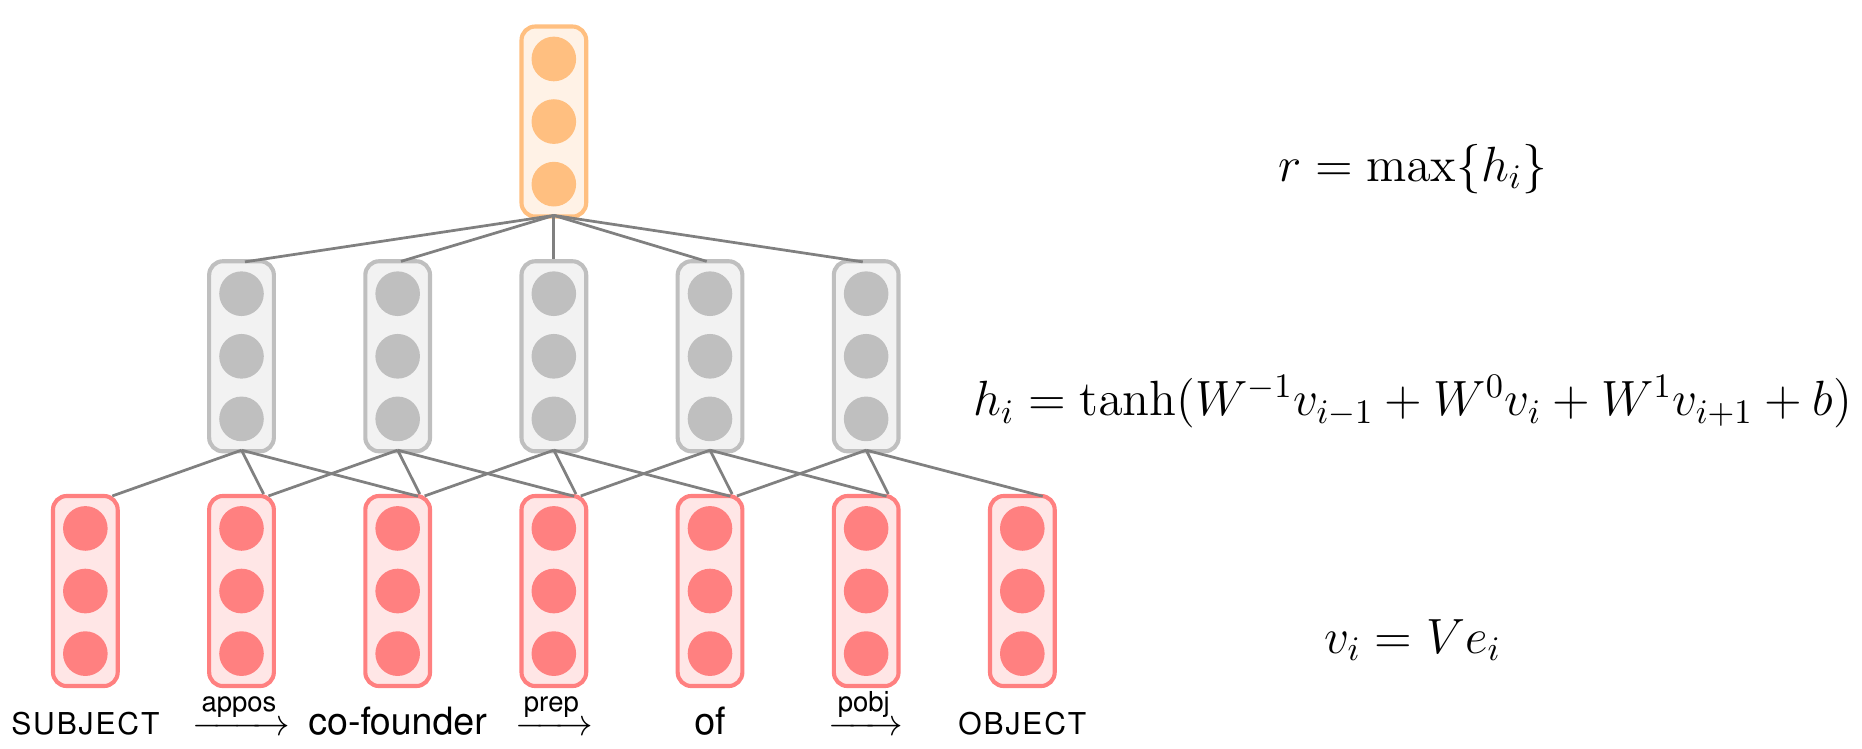
\includegraphics[width=0.85\hsize]{pic/conv.png}
\end{frame}



\frame{
  \begin{columns}[c]
   \column{.15\hsize}
   \column{.7\hsize}
   \begin{block}{}
    \centering \Large 实验  \\ 
   \end{block}
   \column{.15\hsize}
  \end{columns}
}

\begin{frame}{实验}
 \begin{columns}
  \column{0.4\hsize}
 \begin{block}{\alert{KB:}FB15k-237}
  FB15k的子集,237种关系
 \end{block}
  \column{0.4\hsize}
 \begin{block}{\alert{text:}ClueWeb12}
  覆盖了13.9k/14.5k个实体
 \end{block}
 \end{columns}
   \centering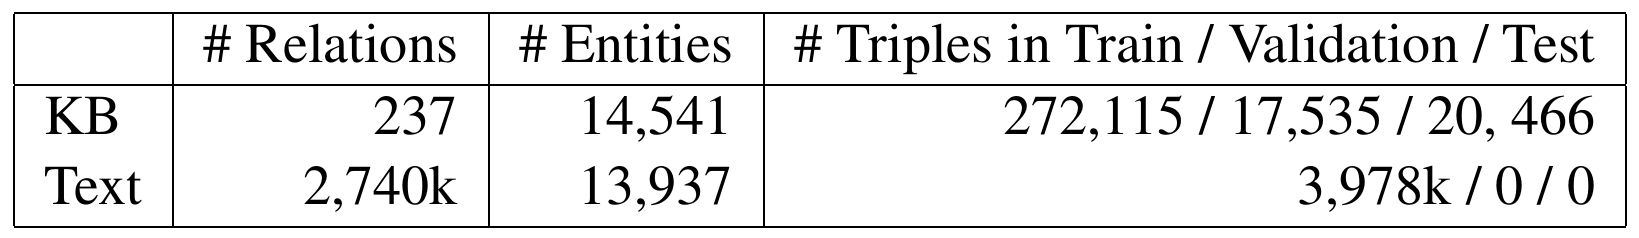
\includegraphics[width=0.85\hsize]{pic/data.png}
   
   \begin{itemize}
   \only<1>{
    \item 可以极大提高F模型学习实体对向量的效果
   \begin{itemize}\footnotesize
    \item 降低稀疏度
    \item 训练集/开发集/测试集中40\%/26\%/28\%的(主语,客体)实体对在ClueWeb中出现
    \item 上面开发集的26\%的实体对中有18\%在训练集中出现,所以有5\%的可能实体对在训练集看过,比不用文本的概率提高了50倍
   \end{itemize}
   }
   \only<2>{
    \item 剪枝策略
      \begin{itemize}
       \item 只有满足relation客体类别的实体才会被纳入候选(去除完全不可能的实体)
       \item 如果实体在训练、开发、测试集 中出现,则不会被纳入候选
	\begin{itemize}
	 \item 这些实体可能是正确的,会导致想要的答案没有排在第一位
	\end{itemize}
      \end{itemize}
   \item 训练时每个三元组选取200个负样本,权重变量$\tau=0.25$,向量维度为10时,效果最好
   }
   \end{itemize}
\end{frame}

\begin{frame}{实验——参数选择}
   \centering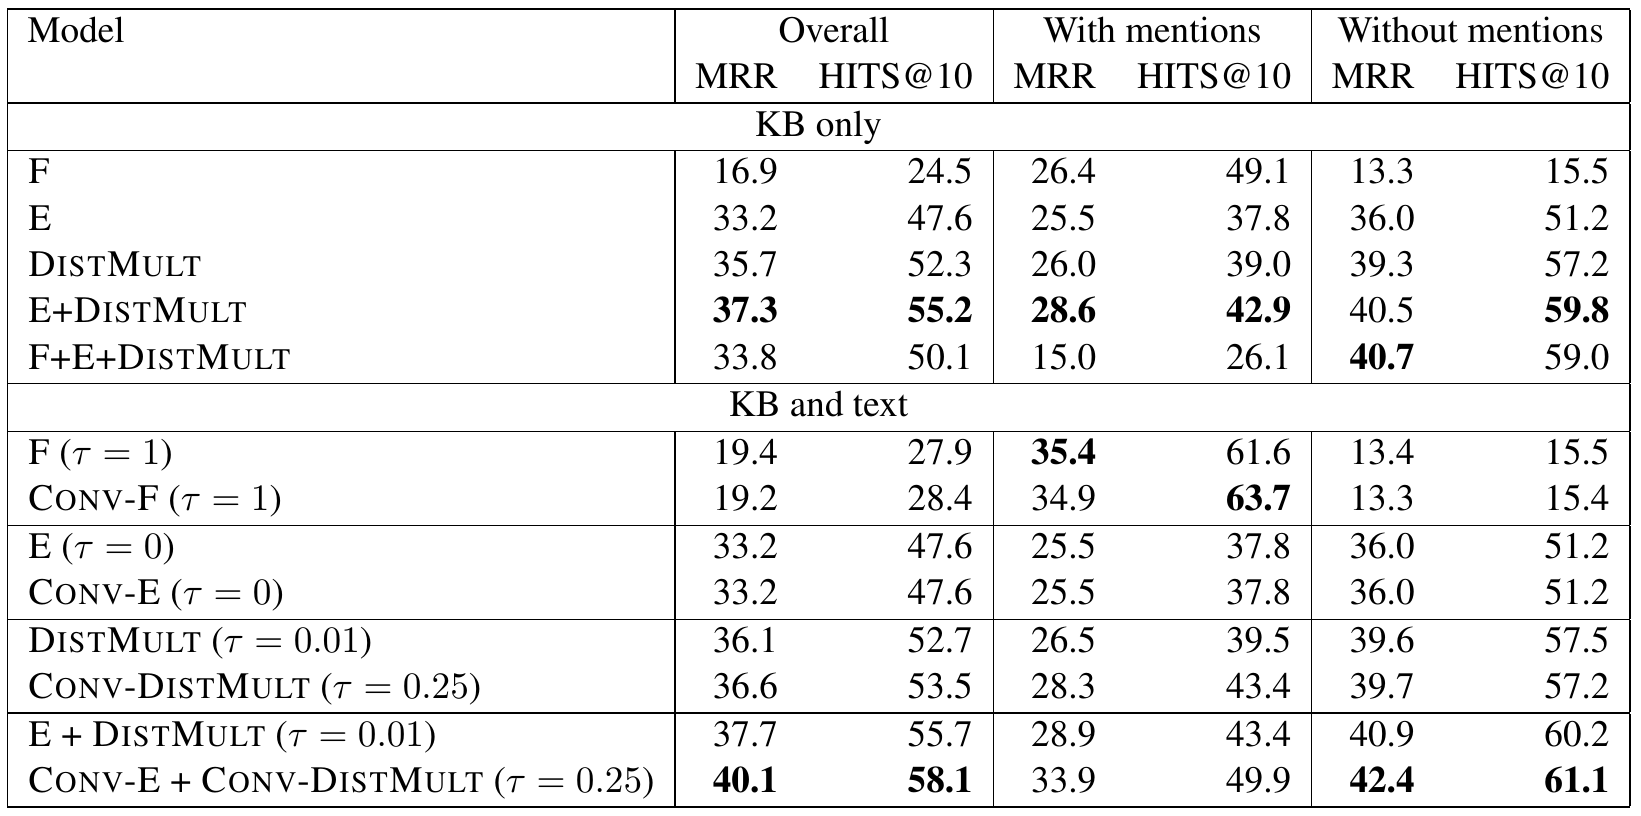
\includegraphics[width=0.85\hsize]{pic/test.png}

  \begin{itemize}\footnotesize
  \only<1>{
   \item with mentions:测试集中的实体对在text中出现过
   \item \textbf{非F模型的第三、第二列好像弄反了}
   \item 对于F模型,只训练在text中出现的实体对(减小复杂度)
   }
   \only<2>{
   \item F的实体对太稀疏,表现不好
   \item E的效果比较好,但是实际上和主语没关系,所以效果不如DISTMULT
   \item E+DISTMULT最好
   }
   \only<3->{
   \item 如果使用text信息\\ 
   \item CONV对E没有提升,对DISTMULT有小提升
   \item 随机初始化的词向量(40.3\%)和使用从KB-only训练出的词向量效果(38.7\%)差别较大
   \item CNN的窗口大小影响不大
   }
  \end{itemize}
\end{frame}


\begin{frame}{相关研究}
  \begin{itemize}
  \item F模型和E、DISTMULT模型不是一回事
   \item F太稀疏了,应该填得更满一些
   \begin{itemize}
  \item NACCL2015 Injecting Logical Background for Relation Extraction
  \item 通过自动的挖掘KB里面的高可信度的一阶逻辑(比如$professorAt(x,y)\Rightarrow emplyeeAt(x,y)$来“填充”稀疏的矩阵)
 \end{itemize}
 
  \end{itemize}

 

\end{frame}




\end{document} 